\hojaejercicio{Transformaciones de Möbius}

% Ejercicio 1
\ejercicio{¿La conjugación es una transformación de Möbius?}{
    No, ya que no es una función holomorfa, y tiene infinitos puntos fijos (la recta real), pero no es la identidad.
}

% Ejercicio 2
\ejercicio{
    Probar que si una transformación de Möbius transforma $\mathbb{R}$ en $\mathbb{R}$, entonces los coeficientes son reales.
}{
    Recordemos que una transformación de Möbius es de la forma:
    \[
    T(z) = \frac{az + b}{cz + d}
    \]
    Sabemos que si $c=0$ $\exists \alpha \neq \beta \in \mathbb{R}: \begin{cases} T(\alpha) = 0 \\ T(\beta) = 1 \\ T(\infty) = \infty \end{cases}$. Entonces:
    \[
    T(z) = \frac{z - \alpha}{\beta - \alpha}
    \]
    Por lo que claramente $T(\mathbb{R}) \subset \mathbb{R}$ y los coeficientes son reales.
    Por otro lado, si $c \neq 0$ sabemos que:
    \[
    \exists \alpha, \beta, \gamma \in \overline{\mathbb{R}} :
    \begin{cases}
        T(\alpha) = 0 \\
        T(\beta) = 1 \\
        T(\gamma) = \infty
    \end{cases} \implies
    \begin{cases}
        \gamma = \infty \implies T(z) = \frac{z - \alpha}{\beta - \alpha} \text{(análogo al caso anterior)}\\
        \gamma \neq \infty \implies 
        \begin{cases}
            \alpha = \infty \implies T(z) = \frac{\beta - \gamma}{z - \gamma}\\
            \alpha \neq \infty \implies T(z) = \frac{(z - \alpha)(\beta - \gamma)}{(z - \gamma)(\beta - \alpha)}
        \end{cases}
    \end{cases}
    \]
}

% Ejercicio 3
\ejercicio{
    Encuentra la transformación de Möbius que transforma:
    \[
    \begin{cases}
        T(0) = 1 \\
        T(i) = -1 \\
        T(-i) = 0
    \end{cases}
    \]
}{
    Despejando el sistema obtenemos:
    \[
    T(z) = \frac{-iz + 1}{3iz + 1}
    \]
    Tambíen la podemos obtener de la siguiente corma:
    \[
    \begin{array}{ccccc}
        & S_{0,i,-i} & & S_{1,-1,0} & \\
        0 & \longrightarrow & 1 & \longleftarrow & 1 \\
        i & \longrightarrow & 0 & \longleftarrow & -1 \\
        -i & \longrightarrow & \infty & \longleftarrow & 0 \\
    \end{array}
    \]
    Por lo que:
    \[
    T(z) = (S_{1,-1,0})^{-1} \circ S_{0,i,-i}(z)
    \]
    Con:
    \[
    S_{0,i,-i}(z) = \frac{\frac{z - i}{z + i}}{\frac{-i}{i}},\quad
    (S_{1,-1,0})^{-1}(w) = \frac{w - 1}{w + 1}
    \]
}

% Ejercicio 4
\ejercicio{
    ¿Cual es la transformación de Möbius que transforma $S(0;2) = \{ z \in \mathbb{C} : |z| = 2 \}$ en $S(-1;1)$, y que tambien $T(-2) = 0$ y $T(0) = i$?
}{
    Sabemos que $\infty$ es simetrico a $0$ con respecto a $C(0;1)$, por lo que $T(\infty)$ es simetrico a $T(0) = i$ respecto de $T(C(0;1)) = C(-1;1)$, por lo que $T(\infty) = -\frac{1}{2} + \frac{i}{2}$, por lo que:
    \[
    T(z) = \frac{
        \frac{z+2}{z - (-\frac{1}{2} + \frac{i}{2})}
    }
    {
        \frac{2}{\frac{1}{2} - \frac{i}{2}}
    }
    = \frac{(-1 + i)z + (2 -i)}{-2z - (2i + 2)}
    \]
}

% Ejercicio 5
\ejercicio{
    ¿Que transformación de Möbius transforma $S(0;1), S(\frac{1}{4}; \frac{1}{4})$ en circunferencias concéntricas?\\
    \textbf{Indicación: } $z^*$ es simétrico de $z$ respecto de la circunferencia $S(0;r)$ si y solo si $z^* \overline{z} = r^2$.
}{
    Aplicamos la indicación para llegar a que $z^*, z$ son simétricos respecto de $S(0;1)$ si:
    \[
    (z^* - z_0) \overline{(z - z_0)} = r^2
    \]
    \textbf{Anotación:} Dada $S(z_0;r)$, la circunferencia de radio $r$, centro $z_0$ y dado un punto $b \in \mathbb{C}$, el simétrico de $b$ respecto de $S(z_0;r)$ es 
    aquel punto $b^*$ que está en la recta que une $z_0$ y $b$ y cumple $|b-z_0||b^* - z_0| = r^2$. Esto se obtiene de la definición de simetría respecto de una circunferencia formal:
    Si $b$ y $b^*$ son simétricos respecto de $S(z_0;r)$, entonces sea $z_1$, $z_2$, $z_3$ una parametrización de $S(z_0;r)$, entonces:
    $(b, z_1, z_2, z_3) = \overline{(b^*, z_1, z_2, z_3)}$.
    (Construyendo la transformación y desarrollando se llega a la misma conclusión).
    \\
    Busquemos puntos simétricos de ambas circunferencias, $S_1$ y $S_2$. Esto lo hacemos porque
    los únicos puntos simétricos comunes a dos circunferencias concéntricas en $0$ (puede ser cualquier $z \in \mathbb{C}$, pero 
    es indiferente, encontramos $T$ que la lleve a dos concéntricas con centro $0$ y luego aplicamos una traslación) son $0$ e $\infty$.
    Entonces, por el principio de simetría, los puntos simétricos de $S_1$ se transforman en los puntos simétricos de $S_2$, es decir, los puntos simétricos
    comunes a ambas circunferencias se transforman en los puntos simétricos comunes a las dos circunferencias concéntricas, es decir, en el centro y el infinito.
    \\
    Lógicamente, los puntos simétricos en común de ambas están en la recta que los une,
    es decir, $\mathbb{R}$ (en este caso particular, ya que ambas circunferencias son concéntricas en $0$).
    Tenemos que resolver entonces, usando la definición de simetría respecto de una circunferencia, el siguiente sistema:
  \[
    \begin{cases}
        (x^* - 0) \overline{(x - 0)} = 1^2 \\
        (x^* - \frac{1}{4}) \overline{(x - \frac{1}{4})} = \left(\frac{1}{4}\right)^2
    \end{cases}\\
    \implies
    \begin{cases}
        x^* x = 1 \\
        (x^* - \frac{1}{4})(x - \frac{1}{4}) = \frac{1}{16}
    \end{cases}
    \implies
    \begin{cases}
    x^*=\frac{1}{x}
    x^2-4x+1=0
    \end{cases}
    \implies
    \begin{cases}
    x^*=\frac{1}{x}
    x=2 + \sqrt{3}
    \end{cases}
    \]  
    Por lo que los puntos simétricos comunes a ambas circunferencias son $2+\sqrt{3}$ y $2-\sqrt{3}$.
    \\  
    Entonces, buscamos la transformación de Möbius que lleva un punto a $0$, otro a $\infty$ y otro, cualquiera a $1$.
    $T(z)= \frac{z-(2+\sqrt{3})}{z-(2-\sqrt{3})}$
    Lleva a $S_1$ y $S_2$ en circunferencias, puesto que no contienen el punto que va al infinito y ambas tienen como simétrico del $\infty$ el $0$ (con centro en 0).
}

%ejercicio 6
\ejercicio{
Determina la transformación de Möbius que transforma el semiplano superior en el disco unidad, el i a 0, el 0 a 1. 
}
{
    Si transformamos la recta real en el círculo unidad, de tal forma que el interior del semiplano superior vaya al interior del disco unidad, tenemos que entonces:
     mandamos $i \mapsto 0$, $0 \mapsto 1$, $-i \mapsto \infty$ (por el principio de simetría, mandamos simétricos de $\mathbb{R}$ en simetricos de D(0,1)).
     Entonces la recta real $\mathbb{R}$ se transforma en un círculo ($\infty \notin T(\mathbb{R})$) y el 
     semiplano superior dentro del disco (puedes comprobarlo parametrizando y utilizar
     el principio de orientación o simplemente viendo que $T(i) = 0$ está dentro del disco unidad). Nuestra transformación es:
    \[
    T(z) = \frac{-z + i}{z + i}
    \]

}
%ejercicio 7
\ejercicio{
¿Cuál es la imagen del tercer cuadrante por $T(z) = \frac{z +i}{z - i}$?
}{
El tercer cuadrante es $\{ z \in \mathbb{C} : \text{Re}(z) < 0, \text{Im}(z) < 0 \}$. 
definido entonces por las rectas $\text{Re}(z) = 0$ e $\text{Im}(z) = 0$.
Veamos a donde van estas rectas:
\begin{itemize}
    \item En el caso de $\mathbb{R}$ tenemos que $\infty \notin T(\mathbb{R})$, por lo que $T(\mathbb{R})$ es una circunferencia. 
    Centrada en $T(-i)=0$ (simétrico del infinito respecto te $T(\mathbb{R})$, i y -i son simétricos respecto de $\mathbb{R}$) y de radio 1 (ya que $T(0)= -1$). 
    \item En el caso de $i\mathbb{R}$ tenemos que $\infty \in T(i\mathbb{R})$ (ya que $T(i) = \infty$), por lo que $T(i\mathbb{R})$ es una recta, que
    pasa por el 0 ($T(-i) = 0$) y por el -1 ($T(0) = -1$).
\end{itemize} 
Es claro entonces que, como  $-1-i$(del tercer cuadrante) tiene imagen 
$T(-1-i) = \frac{-1}{-1-2i} = \frac{1-2i}{5}$ dentro de la circunferencia y debajo la recta, la imagen del tercer cuadrante es el sector 
delimitado por la circunferencia de centro $0$ y radio $1$ y la recta real.

}
%ejercicio 8
\ejercicio{
    Hallar la imagen de $z\in \mathbb{C}$ / $\frac{-\pi}{4}<Arg(z)<\frac{\pi}{4}$ por la transformación de Möbius $T(z) = \frac{z}{z - 1}$.
}
{
    $T(z) = \frac{z}{z - 1}$ tiene coeficientes reales, por lo que transforma la recta real en si misma ($T(\mathbb{R}) = \mathbb{R}$).
    El punto que va a $\infty$ es $1$, por lo que la recta real se transforma en una recta. Las dos rectas que definen el conjunto
    que son 
    \[
    r1: \Im(z)=\Re(z), \quad
    r2: \Im(z)=-\Re(z)
    \] 
    se transforman en dos circunferencias ($\infty \notin T(r1)$ y $\infty \notin T(r2)$).
    \\
Los centros de las circunferencias son los simétricos de $\infty$ respecto a ellas mismas. Es decir que, por una transformacion de Möbius deben de ser los simétricos de 1 respecto a r1 y r2.
    \\
    El simétrico de 1 respecto a r1 es $i$ y el simétrico de 1 respecto a r2 es $-i$. Por lo que las circunferencias son
    \begin{itemize}
        \item C1: centro $T(i)$ radio $|T(i)-T(0)|$ 
        \item C2: centro $T(-i)$ radio $|T(-i)-T(0)|$.
    \end{itemize} 
    Viendo que 2 está en la región dada por las dos rectas, y que su imagen $T(2) = 2$ está 
    fuera de las dos circunferencias, la imagen del conjunto es $\mathbb{C}$ menos el interior de las dos circunferencias.

    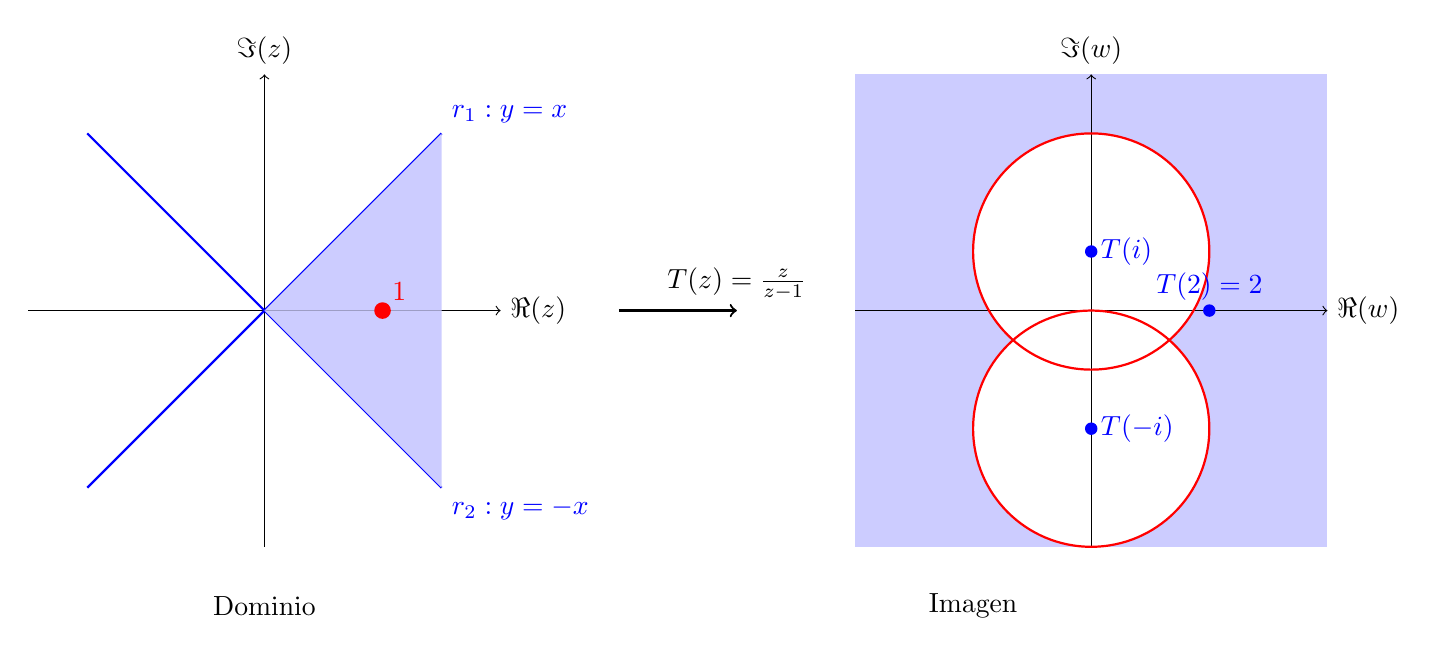
\begin{tikzpicture}[scale=1.5]
    % Grid y ejes para el dominio (izquierda)
    \begin{scope}[xshift=-4cm]
        % Ejes
        \draw[->] (-2,0) -- (2,0) node[right] {$\Re(z)$};
        \draw[->] (0,-2) -- (0,2) node[above] {$\Im(z)$};
        
        % Rectas que definen el sector angular
        \draw[blue, thick] (-1.5,-1.5) -- (1.5,1.5) node[above right] {$r_1: y=x$};
        \draw[blue, thick] (-1.5,1.5) -- (1.5,-1.5) node[below right] {$r_2: y=-x$};
        
        % Sector sombreado
        \fill[blue!20] (0,0) -- (1.5,1.5) -- (1.5,0) -- cycle;
        \fill[blue!20] (0,0) -- (1.5,-1.5) -- (1.5,0) -- cycle;
        
        % Punto singular z=1
        \fill[red] (1,0) circle (2pt) node[above right] {$1$};
        
        \node at (0,-2.5) {Dominio};
    \end{scope}
    
    % Flecha de transformación
    \draw[->, thick] (-1,0) -- (0,0) node[above] {$T(z)=\frac{z}{z-1}$};
    
    % Grid y ejes para la imagen (derecha)
    \begin{scope}[xshift=2cm]
         % Sombreado exterior (región imagen)
        %\clip (-1,-2) rectangle (3,2);
        \fill[blue!20] (-1,-2) rectangle (3,2);
        \fill[white] (1,0.5) circle (1);
        \fill[white] (1,-1) circle (1);
        % Ejes
        \draw[->] (-1,0) -- (3,0) node[right] {$\Re(w)$};
        \draw[->] (1,-2) -- (1,2) node[above] {$\Im(w)$};
        
        % Circunferencias imagen
        \draw[red, thick] (1,0.5) circle (1); % C1 centrada en i
        \draw[red, thick] (1,-1) circle (1); % C2 centrada en -i
        
       
        
        % Puntos especiales
        \fill[blue] (2,0) circle (1.5pt) node[above] {$T(2)=2$};
        \fill[blue] (1,0.5) circle (1.5pt) node[right] {$T(i)$};
        \fill[blue] (1,-1) circle (1.5pt) node[right] {$T(-i)$};
        
        \node at (0,-2.5) {Imagen};
    \end{scope}
\end{tikzpicture}
}
%ejercicio 9
\ejercicio{
    Halla la imagen de $\{z \in \mathbb{C} : \Im(z) > 0\} \setminus \{z \in \mathbb{C}: |z|<1\}$ por $T(z) = \frac{z+1}{z - 1}$.
}{
Como $T$ es biyectiva, la imagen del conjunto es el conjunto imagen menos la imagen del conjunto eliminado.
Tenemos dos conjuntos a transformar:
\[
C=\{z \in \mathbb{C} : \Im(z)=0\}\text{ y } D=\{z \in \mathbb{C}: |z|=1\}
\]
\[
\begin{cases}
T(1)=\infty \text{ (por lo que $T(C)$ es una recta)},  \\
T(\infty)=1\\
T(0)=-1
\end{cases}
\]

Entonces $T(C)$ es la recta real.
(también es lógico teniendo en cuenta que al tener coeficientes reales, los valores reales se transforman en valores reales).
\\
Para transformar $D$, usamos el principio de simetría. Sabemos que $T(\infty)=1$ $\longleftrightarrow$
el simétrico de $1$ respecto a $T(D)$ es $T(0)=-1$.
Como $T(1)=\infty$, entonces $T(D)$ es una recta (pasa por el infinito),
respecto a la cual $1$ y $-1$ son simétricos 
$\longleftrightarrow$ $T(D)$ es la recta imaginaria.
\\
Cogemos $1+i$ (que está en el conjunto original) y 
vemos que su imagen es $T(1+i) = \frac{2+i}{i} = 1 - 2i$, 
que está en el IV cuadrante.
Por lo que la imagen del conjunto es:
\[
\{w \in \mathbb{C} : \Im(w) < 0\} \setminus \{w \in \mathbb{C} : \Re(w)<0\}
\]
\begin{tikzpicture}[scale=1.1]

% =====================
% PANEL IZQUIERDO: Dominio
% =====================
\begin{scope}[shift={(-4.5,0)}]
    % Ejes
    \draw[->] (-2.5,0) -- (2.5,0) node[right] {$\Re(z)$};
    \draw[->] (0,-0.5) -- (0,2.5) node[above] {$\Im(z)$};
    
    % Región Im(z) > 0
    \fill[blue!10] (-2.5,0) rectangle (2.5,2.5);
    
    % Círculo |z|=1
    \draw[thick,red] (0,0) circle (1);
    
    % Región excluida |z|<1
    \fill[white] (0,0) circle (1);
    \draw[red,dashed] (0,0) circle (1);
    
    % Etiquetas
    \node[blue!70!black] at (1.2,1.5) {$\Im(z)>0$};
    \node[red!70!black] at (1.5,0.3) {$|z|<1$};
    \node at (0,-0.3) {$0$};
    \node at (1.1,-0.3) {$1$};
    \node at (-1.1,-0.3) {$-1$};
    
    \node[below] at (0,-1) {\small Conjunto original en $z$};
\end{scope}

% =====================
% PANEL DERECHO: Imagen
% =====================
\begin{scope}[shift={(4.5,0)}]
    % Ejes
    \draw[->] (-2.5,0) -- (2.5,0) node[right] {$\Re(w)$};
    \draw[->] (0,-2.5) -- (0,2.5) node[above] {$\Im(w)$};
    
    % Región Im(w) < 0
    \fill[blue!10] (-2.5,-2.5) rectangle (2.5,0);
    
    % Semiplano excluido Re(w) < 0
    \fill[white] (-2.5,-2.5) rectangle (0,0);
    \draw[dashed,red] (0,-2.5) -- (0,2.5);
    
    % Etiquetas
    \node[blue!70!black] at (1.5,-1.5) {$\Im(w)<0$};
    \node[red!70!black] at (-1.3,1.8) {$\Re(w)<0$};
    \node at (0.3,0.2) {$0$};
    \node at (1.1,0.2) {$1$};
    \node at (-1.1,0.2) {$-1$};
    
    % Imagen de 1+i
    \filldraw[black] (1,-2) circle (1.5pt);
    \node[right] at (1,-2) {$T(1+i)=1-2i$};
    
    \node[below] at (0,-3) {\small Imagen bajo $T(z)=\dfrac{z+1}{z-1}$};
\end{scope}

% Flecha de transformación
\draw[->,thick] (-1,0) -- (1,0) node[midway,above] {$T$};

\end{tikzpicture}
}
%ejercicio 10
\ejercicio{
    Encuentra dos transformaciones de Möbius que transformen $S(i+1;1)$ en $\mathbb{R}$.¿Cuál es la imagen de 1+i en cada caso?

}{
La recta real cumple que tiene a -i e i como simétricos, además de que  $\infty \in \mathbb{R}$. Por lo tanto, las transformaciones:
\[
\begin{cases}
T_1(0)=i\\
T_1(\infty)=-i\\
T_1(1+i)= \infty
\end{cases}
\Longrightarrow T_1(z)= \frac{-iz-i(1+i)}{z - (1+i)} 
\\
\text{ y }\\
\begin{cases}
T_2(0)=i\\
T_2(\infty)=-i\\
T_2(1)=\infty
\end{cases}
\Longrightarrow
T_2(z)= \frac{(-iz-i)}{(z - 1)} 
\]
\\
Transforman circunferencias de centro 0 y radio 1 en la recta real.
Por lo tanto, trasladamos $S(i+1;1)$ a $S(0;1)$ y aplicamos $T_1$ o $T_2$.\\
Es decir:\\
\[
T^*_1(z) =T(z-1-i)= \frac{-i(z-1-i)-i(1+i)}{(z-1-i) - (1+i)} = \frac{-iz}{z -2 -2i}
\]
\[
T^*_2(z) =T(z-1-i)= \frac{-i(z-1-i)-i}{(z-1-i) - 1} = \frac{-iz -1}{z - i-2}
\]
\\


En el primer caso, $T^*_1(1+i) = i$, y en el segundo caso, $T^*_2(1+i) = i$.
}
